\documentclass[]{article}
\usepackage{lmodern}
\usepackage{amssymb,amsmath}
\usepackage{ifxetex,ifluatex}
\usepackage{fixltx2e} % provides \textsubscript
\ifnum 0\ifxetex 1\fi\ifluatex 1\fi=0 % if pdftex
  \usepackage[T1]{fontenc}
  \usepackage[utf8]{inputenc}
\else % if luatex or xelatex
  \ifxetex
    \usepackage{mathspec}
  \else
    \usepackage{fontspec}
  \fi
  \defaultfontfeatures{Ligatures=TeX,Scale=MatchLowercase}
\fi
% use upquote if available, for straight quotes in verbatim environments
\IfFileExists{upquote.sty}{\usepackage{upquote}}{}
% use microtype if available
\IfFileExists{microtype.sty}{%
\usepackage{microtype}
\UseMicrotypeSet[protrusion]{basicmath} % disable protrusion for tt fonts
}{}
\usepackage[margin=1in]{geometry}
\usepackage{hyperref}
\hypersetup{unicode=true,
            pdftitle={CEU Unstructured Text Analysis Seminar - Assignment},
            pdfauthor={Imre Boda},
            pdfborder={0 0 0},
            breaklinks=true}
\urlstyle{same}  % don't use monospace font for urls
\usepackage{color}
\usepackage{fancyvrb}
\newcommand{\VerbBar}{|}
\newcommand{\VERB}{\Verb[commandchars=\\\{\}]}
\DefineVerbatimEnvironment{Highlighting}{Verbatim}{commandchars=\\\{\}}
% Add ',fontsize=\small' for more characters per line
\usepackage{framed}
\definecolor{shadecolor}{RGB}{248,248,248}
\newenvironment{Shaded}{\begin{snugshade}}{\end{snugshade}}
\newcommand{\KeywordTok}[1]{\textcolor[rgb]{0.13,0.29,0.53}{\textbf{{#1}}}}
\newcommand{\DataTypeTok}[1]{\textcolor[rgb]{0.13,0.29,0.53}{{#1}}}
\newcommand{\DecValTok}[1]{\textcolor[rgb]{0.00,0.00,0.81}{{#1}}}
\newcommand{\BaseNTok}[1]{\textcolor[rgb]{0.00,0.00,0.81}{{#1}}}
\newcommand{\FloatTok}[1]{\textcolor[rgb]{0.00,0.00,0.81}{{#1}}}
\newcommand{\ConstantTok}[1]{\textcolor[rgb]{0.00,0.00,0.00}{{#1}}}
\newcommand{\CharTok}[1]{\textcolor[rgb]{0.31,0.60,0.02}{{#1}}}
\newcommand{\SpecialCharTok}[1]{\textcolor[rgb]{0.00,0.00,0.00}{{#1}}}
\newcommand{\StringTok}[1]{\textcolor[rgb]{0.31,0.60,0.02}{{#1}}}
\newcommand{\VerbatimStringTok}[1]{\textcolor[rgb]{0.31,0.60,0.02}{{#1}}}
\newcommand{\SpecialStringTok}[1]{\textcolor[rgb]{0.31,0.60,0.02}{{#1}}}
\newcommand{\ImportTok}[1]{{#1}}
\newcommand{\CommentTok}[1]{\textcolor[rgb]{0.56,0.35,0.01}{\textit{{#1}}}}
\newcommand{\DocumentationTok}[1]{\textcolor[rgb]{0.56,0.35,0.01}{\textbf{\textit{{#1}}}}}
\newcommand{\AnnotationTok}[1]{\textcolor[rgb]{0.56,0.35,0.01}{\textbf{\textit{{#1}}}}}
\newcommand{\CommentVarTok}[1]{\textcolor[rgb]{0.56,0.35,0.01}{\textbf{\textit{{#1}}}}}
\newcommand{\OtherTok}[1]{\textcolor[rgb]{0.56,0.35,0.01}{{#1}}}
\newcommand{\FunctionTok}[1]{\textcolor[rgb]{0.00,0.00,0.00}{{#1}}}
\newcommand{\VariableTok}[1]{\textcolor[rgb]{0.00,0.00,0.00}{{#1}}}
\newcommand{\ControlFlowTok}[1]{\textcolor[rgb]{0.13,0.29,0.53}{\textbf{{#1}}}}
\newcommand{\OperatorTok}[1]{\textcolor[rgb]{0.81,0.36,0.00}{\textbf{{#1}}}}
\newcommand{\BuiltInTok}[1]{{#1}}
\newcommand{\ExtensionTok}[1]{{#1}}
\newcommand{\PreprocessorTok}[1]{\textcolor[rgb]{0.56,0.35,0.01}{\textit{{#1}}}}
\newcommand{\AttributeTok}[1]{\textcolor[rgb]{0.77,0.63,0.00}{{#1}}}
\newcommand{\RegionMarkerTok}[1]{{#1}}
\newcommand{\InformationTok}[1]{\textcolor[rgb]{0.56,0.35,0.01}{\textbf{\textit{{#1}}}}}
\newcommand{\WarningTok}[1]{\textcolor[rgb]{0.56,0.35,0.01}{\textbf{\textit{{#1}}}}}
\newcommand{\AlertTok}[1]{\textcolor[rgb]{0.94,0.16,0.16}{{#1}}}
\newcommand{\ErrorTok}[1]{\textcolor[rgb]{0.64,0.00,0.00}{\textbf{{#1}}}}
\newcommand{\NormalTok}[1]{{#1}}
\usepackage{graphicx,grffile}
\makeatletter
\def\maxwidth{\ifdim\Gin@nat@width>\linewidth\linewidth\else\Gin@nat@width\fi}
\def\maxheight{\ifdim\Gin@nat@height>\textheight\textheight\else\Gin@nat@height\fi}
\makeatother
% Scale images if necessary, so that they will not overflow the page
% margins by default, and it is still possible to overwrite the defaults
% using explicit options in \includegraphics[width, height, ...]{}
\setkeys{Gin}{width=\maxwidth,height=\maxheight,keepaspectratio}
\IfFileExists{parskip.sty}{%
\usepackage{parskip}
}{% else
\setlength{\parindent}{0pt}
\setlength{\parskip}{6pt plus 2pt minus 1pt}
}
\setlength{\emergencystretch}{3em}  % prevent overfull lines
\providecommand{\tightlist}{%
  \setlength{\itemsep}{0pt}\setlength{\parskip}{0pt}}
\setcounter{secnumdepth}{0}
% Redefines (sub)paragraphs to behave more like sections
\ifx\paragraph\undefined\else
\let\oldparagraph\paragraph
\renewcommand{\paragraph}[1]{\oldparagraph{#1}\mbox{}}
\fi
\ifx\subparagraph\undefined\else
\let\oldsubparagraph\subparagraph
\renewcommand{\subparagraph}[1]{\oldsubparagraph{#1}\mbox{}}
\fi

%%% Use protect on footnotes to avoid problems with footnotes in titles
\let\rmarkdownfootnote\footnote%
\def\footnote{\protect\rmarkdownfootnote}

%%% Change title format to be more compact
\usepackage{titling}

% Create subtitle command for use in maketitle
\newcommand{\subtitle}[1]{
  \posttitle{
    \begin{center}\large#1\end{center}
    }
}

\setlength{\droptitle}{-2em}
  \title{CEU Unstructured Text Analysis Seminar - Assignment}
  \pretitle{\vspace{\droptitle}\centering\huge}
  \posttitle{\par}
  \author{Imre Boda}
  \preauthor{\centering\large\emph}
  \postauthor{\par}
  \predate{\centering\large\emph}
  \postdate{\par}
  \date{2018-03-30T21:13:14-05:00}


\begin{document}
\maketitle

\section{Introduction}\label{introduction}

This is my term assignment of the Unstructured Text Analysis Seminar at
CEU in the 2018 winter semester. The course was held by Mr.~Eduardo
Arino de la Rubia. The assignment was about to create something that use
the stuff taught and learnt in the course. I used a lot from the
techniques described in the great book ``Text Mining with R'' by Julia
Silge and David Robinson.

My work is a Facebook post and comment analyzer shiny dashboard. It
looks at the Facebook pages of a few telco and related vendors (to some
extent related to telcos' traditional or new business segments), and
presents / compares their key marketing themes during the past few
quarters. Also, looks at the comments to the posts and does a sentiment
analysis on the them along the time. At the time of writing this blog,
the program is hosted at AWS, available at
\url{http://boda.ceudata.net:3838/}.

The dashboard consists of 3 main parts:

\begin{itemize}
\tightlist
\item
  Presenting the key post themes of the selected vendor per quarter,
\item
  Compares the key Facebook themes of the selected vendors to a
  benchmark vendor,
\item
  Shows the sentiment scores of the two vendors along time.
\end{itemize}

Key Facebook ``themes'' in this context are the most often used phrases
(words and bi-grams). When I played with more sophisticated algorithms
(tf-idf, LDA), they showed no better result. Maybe this is due to the
nature of these posts, so finally I stayed with this simple way.

Sentiment scoring is based on summing up the words with positive /
negative sentiment load, correcting it with a bi-gram sentiment check
(making sure that terms such as ``not nice'' are properly calculated as
negative not as positive).

\begin{figure}[htbp]
\centering
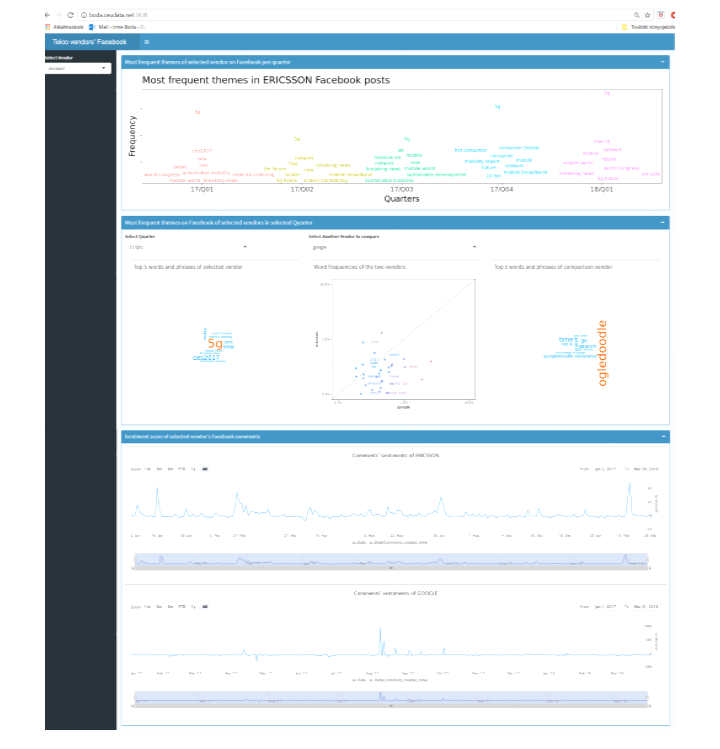
\includegraphics{/img/Dashboard.png}
\caption{Dashboard screenshot.}
\end{figure}

The main steps of the works were the followings:

\begin{itemize}
\tightlist
\item
  Setting up the infrastructure on AWS,
\item
  Obtaining Facebook token,
\item
  Writing a script that pulls, stores and analyses posts \& comments
  from Facebook,
\item
  Scheduling daily execution in Jenkins,
\item
  Creating the shiny app.
\end{itemize}

\section{Setting up the infrastructure on
AWS}\label{setting-up-the-infrastructure-on-aws}

It consisted of the following steps:

\begin{itemize}
\tightlist
\item
  Creating EC2 instance with Ubuntu,
\item
  In the ``Security Group'' settings opening ports for Rstudio, Jenkins
  and Shiny,
\item
  Installing RStudio, creating RStudio admin user on Ubuntu
\item
  Installing shiny and shiny server,
\item
  Installing R packages from the command line in order to make them
  available for all R users (needed for script scheduled from Jenkins),
\item
  Installing Jenkins, customizing, creating Jenkins admin user.
\end{itemize}

\section{Obtaining a Facebook token}\label{obtaining-a-facebook-token}

Fairly short, but for a Facebook analysis obviously inevitable workflow:

\begin{itemize}
\tightlist
\item
  Registering at Facebook Developer page
  (\url{https://developers.Facebook.com}),
\item
  Creating a new App, getting the App ID and App Secret,
\item
  On Facebook App login setting site URL of the App to
  ``\url{http://localhost:1410/}'',
\item
  From Rstudio (with Rfacebook installed), starting fboAuth with the App
  ID and App Secret parameters obtained in the previous step,
\item
  Following the instructions seen on the console,
\item
  Saving the received token somewhere for later use.
\end{itemize}

\section{The script that pulls / stores post and comment data from
Facebook}\label{the-script-that-pulls-stores-post-and-comment-data-from-facebook}

This script is run daily, as scheduled from Jenkins. It fetches and
stores Facebook posts and comments of selected vendors. It every night
scrapes all such data for a given period, regardless that all except
last day's info have been collected before. I thought that disregarding
earlier collected data and recollecting again is a cleaner (though not
economic) way then relaying on data gathered and stored before, checking
if that data is fully valid and not corrupted in any way, no new
comments received to earlier posts, etc. Obtaining (dominantly the same)
data every day is more work for machines, but this is why we have
machines. It is cleaner, and after all, the data volume is not super
high, so it causes no disturbance to anyone.

\subsubsection{Fetching, a bit cleaning and transforming data from
Facebook}\label{fetching-a-bit-cleaning-and-transforming-data-from-facebook}

First, it loads the Facebook Authentication token (saved as per the
previous chapter).

Then in the main section from a given date (At the time of writing it is
``2017-01-01''. I don't think I will leave this running for long, but if
I will, then it will be modified to be 5 - 7 quarters back from the
actual date) until the day before, in a cycle it does the following:

\begin{itemize}
\tightlist
\item
  For each vendor's page it reads the posts in 5 days chunks, as the
  number of posts returned in one query has a limit by Facebook.
  Transforms the date info a bit, as some display will be done on a per
  quarter basis, and stores the result in a ``posts table''.
\item
  For each collected post, it reads all comments and stores them in
  another table, the ``comments table''.
\item
  Since many posts do not have message field, but they point to an
  article link with meaningful URL (e.g.
  ``\url{http://www.adweek.com/tv-video/how-watson-is-digging-through-decades-of-video-to-help-find-new-sources-of-revenue/}''),
  the script extracts meaningful info from the URL for such posts with
  empty message field. It searches for patterns that starts with ``/'',
  followed by at least 3 times ``one or more word characters followed by
  -'' then again some word characters (such pattern is
  ``how-watson-is-digging-through-decades-of-video-to-help-find-new-sources-of-revenue/'').
  The reason for requesting at least 3 times of ``word characters plus
  `-'\,'' sequences and then some word characters is to exclude patterns
  like ``/2017-03-01/'', pretty typical in URLs. Such patterns are
  cleaned from leading ``/'' and separator ``-'' characters and copied
  to a new field called ``Headline'', to make up for the empty
  ``message'' field. In vast majority of the cases this seems to do the
  job.
\end{itemize}

\begin{Shaded}
\begin{Highlighting}[]
\NormalTok{### extracting headline from news link, if message is empty}
\NormalTok{VendorPosts_womessage <-}\StringTok{ }\NormalTok{VendorPosts%>%}
\StringTok{    }\KeywordTok{filter}\NormalTok{(}\KeywordTok{is.na}\NormalTok{(message)) %>%}
\StringTok{    }\KeywordTok{mutate} \NormalTok{(}\DataTypeTok{Headline =} \KeywordTok{str_extract} \NormalTok{(link, }\StringTok{"/(}\CharTok{\textbackslash{}\textbackslash{}}\StringTok{w+-)\{3,\}[}\CharTok{\textbackslash{}\textbackslash{}}\StringTok{w]+"}\NormalTok{)) %>%}\StringTok{    }\CommentTok{#search for patterns like "/5g-connected-trials-c.."}
\StringTok{    }\KeywordTok{mutate} \NormalTok{(}\DataTypeTok{Headline =} \KeywordTok{str_replace} \NormalTok{(Headline, }\StringTok{"^/"}\NormalTok{,}\StringTok{""}\NormalTok{)) %>%}\StringTok{   }\CommentTok{#strip leading / }
\StringTok{    }\KeywordTok{mutate} \NormalTok{(}\DataTypeTok{Headline =} \KeywordTok{str_replace_all} \NormalTok{(Headline, }\StringTok{"-"}\NormalTok{, }\StringTok{" "}\NormalTok{)) }
\end{Highlighting}
\end{Shaded}

\begin{itemize}
\tightlist
\item
  For the rest of the posts, which do contain ``message'' info, this
  field is copied to the newly created ``Headline'' column, getting rid
  of potential ``:http\ldots{}'' references, which often appended to the
  end of Facebook posts in the form of ``read more at: http\ldots{}'',
  ``learn more: http\ldots{}'' and alike.
\end{itemize}

\begin{Shaded}
\begin{Highlighting}[]
\NormalTok{### copy message to headline for the rest}
  \NormalTok{VendorPosts_wmessage <-}\StringTok{ }\NormalTok{VendorPosts %>%}\StringTok{ }
\StringTok{    }\KeywordTok{filter}\NormalTok{(!}\KeywordTok{is.na}\NormalTok{(message)) %>%}
\StringTok{    }\KeywordTok{mutate} \NormalTok{(}\DataTypeTok{Headline =} \NormalTok{message) %>%}
\StringTok{    }\KeywordTok{mutate} \NormalTok{(}\DataTypeTok{Headline =} \KeywordTok{str_replace} \NormalTok{(Headline, }\StringTok{"htt.*$"}\NormalTok{, }\StringTok{""}\NormalTok{)) %>%}\StringTok{    }\CommentTok{#remove http.....}
\StringTok{    }\KeywordTok{mutate} \NormalTok{(}\DataTypeTok{Headline =} \KeywordTok{str_replace} \NormalTok{(Headline, }\StringTok{":}\CharTok{\textbackslash{}\textbackslash{}}\StringTok{s*$"}\NormalTok{, }\StringTok{""}\NormalTok{))        }\CommentTok{#remove ": ", mostly inherited from ": http..."}
\end{Highlighting}
\end{Shaded}

This way all real or created messages are placed in column ``Headline'',
(most often) containing the story.

\begin{itemize}
\tightlist
\item
  As mentioned above, messages often contain ``learn more'', ``can
  find'',\ldots{} phrases, which are in this context to be treated as
  junks, so these are filtered out.
\end{itemize}

\begin{Shaded}
\begin{Highlighting}[]
  \NormalTok{VendorPosts <-}\StringTok{ }\NormalTok{VendorPosts %>%}
\StringTok{    }\KeywordTok{mutate} \NormalTok{(}\DataTypeTok{Headline =} \KeywordTok{str_replace_all}\NormalTok{( Headline, }\StringTok{"read more"}\NormalTok{, }\StringTok{""}\NormalTok{)) %>%}
\StringTok{    }\KeywordTok{mutate} \NormalTok{(}\DataTypeTok{Headline =} \KeywordTok{str_replace_all} \NormalTok{(Headline, }\StringTok{"learn more"}\NormalTok{, }\StringTok{""}\NormalTok{)) %>%}
\StringTok{    }\KeywordTok{mutate} \NormalTok{(}\DataTypeTok{Headline =} \KeywordTok{str_replace_all} \NormalTok{(Headline, }\StringTok{"can find"}\NormalTok{, }\StringTok{""}\NormalTok{))}
\end{Highlighting}
\end{Shaded}

\begin{itemize}
\tightlist
\item
  Finally, a mega table creating all posts and relevant comments are
  created with joining ``posts table'' and ``comments table''. The above
  are repeated for all vendors, and the result (posts and comments) are
  stored in ``AllPostsComments''.
\end{itemize}

\begin{Shaded}
\begin{Highlighting}[]
\NormalTok{VendorPosts <-}\StringTok{ }\NormalTok{VendorPosts %>%}\StringTok{ }\KeywordTok{left_join}\NormalTok{(VendorCommentsTable, }\DataTypeTok{by =} \KeywordTok{c}\NormalTok{(}\StringTok{"id"}\NormalTok{=}\StringTok{"PostID"}\NormalTok{))}

  \NormalTok{### Putting to one list  }
\NormalTok{AllPostsComments <-}\StringTok{ }\KeywordTok{rbind} \NormalTok{(AllPostsComments, VendorPosts)}
\end{Highlighting}
\end{Shaded}

The final table is saved in a file, just in any case.

\subsection{Fetching, a bit cleaning and transforming data from
Facebook}\label{fetching-a-bit-cleaning-and-transforming-data-from-facebook-1}

Once all above are done, comes the shallow text mining part, which
consists of two parts:

\begin{itemize}
\tightlist
\item
  Finding the key post themes,
\item
  Sentiment analysis on the comments.
\end{itemize}

\paragraph{Finding key themes in
posts}\label{finding-key-themes-in-posts}

As said above, this is based on simply getting the most frequent words
and bi-grams in the posts. As mentioned in the introduction section, I
played with tf-idf and LDA, but their output was not better than the
simple term frequency, so that was selected for the finally implemented
version.

As themes are presented and compared on a per vendor and per quarter
basis, 5 most frequent words and 5 most frequent bi-grams are to be
marked per quarter per vendor. It is done in two rounds, first for
uni-grams and then for bi-grams. The reason for doing it in two separate
rounds is that naturally word frequencies are higher than bi-gram
frequencies, therefor if top phrases would be collected in one go, only
words could qualify for the top 5 or top 10 places, not bi-grams.

First we get rid of duplicate posts (introduced when we merged ``posts
table'' and ``comments table'', as one post had typically several
comments), word tokenize the ``Headline'' column, get rid of normal
stopwords and special stopwords (containing the vendors' names and some
words that they frequently use in posts so here become junk). An
interesting feature of regexp that even though ``zte's'' was among the
``specific'' stopwords, after the relevant join operation it stayed in
the tokenized table. Therefore an extra filter was put in (see below) to
remove all words that has the structure ``word character(s) followed by
a non-word character then possibly followed by word character(s)''.

Then the words' frequency per vendor per quarter is added to each
remaining word.

\begin{Shaded}
\begin{Highlighting}[]
\NormalTok{tidyPosts <-}\StringTok{ }\NormalTok{AllPostsComments %>%}
\StringTok{  }\KeywordTok{group_by}\NormalTok{(id) %>%}\StringTok{                }\CommentTok{#from here until ungroup: get rid of duplicate posts}
\StringTok{  }\KeywordTok{filter}\NormalTok{(}\KeywordTok{row_number}\NormalTok{() ==}\StringTok{ }\DecValTok{1}\NormalTok{) %>%}
\StringTok{  }\NormalTok{ungroup %>%}
\StringTok{  }\KeywordTok{unnest_tokens} \NormalTok{(word, Headline) %>%}
\StringTok{  }\KeywordTok{filter}\NormalTok{(!}\KeywordTok{is.na}\NormalTok{(word)) %>%}
\StringTok{  }\KeywordTok{anti_join} \NormalTok{(stp_en) %>%}
\StringTok{  }\KeywordTok{anti_join} \NormalTok{(stp_spc) %>%}
\StringTok{  }\KeywordTok{mutate}\NormalTok{(}\DataTypeTok{word =} \KeywordTok{str_replace}\NormalTok{(word, }\StringTok{"}\CharTok{\textbackslash{}\textbackslash{}}\StringTok{w+[^}\CharTok{\textbackslash{}\textbackslash{}}\StringTok{w]}\CharTok{\textbackslash{}\textbackslash{}}\StringTok{w*"}\NormalTok{, }\StringTok{""}\NormalTok{)) %>%}\StringTok{   }\CommentTok{#"zte's" was not propoerly filtered by stp_spc}
\StringTok{  }\KeywordTok{filter}\NormalTok{(word !=}\StringTok{ ""}\NormalTok{) }

\NormalTok{proportion <-}\StringTok{ }\NormalTok{tidyPosts %>%}
\StringTok{  }\KeywordTok{count} \NormalTok{(Vendor, created_Q, word, }\DataTypeTok{sort =} \OtherTok{TRUE}\NormalTok{) %>%}\StringTok{   }\CommentTok{#count words per vendor per Q}
\StringTok{  }\KeywordTok{group_by} \NormalTok{(Vendor, created_Q) %>%}
\StringTok{  }\KeywordTok{mutate} \NormalTok{(}\DataTypeTok{prop =}  \NormalTok{n/}\KeywordTok{sum}\NormalTok{(n) *}\StringTok{ }\DecValTok{100}\NormalTok{) %>%}
\StringTok{  }\KeywordTok{arrange} \NormalTok{(}\KeywordTok{desc}\NormalTok{(prop)) %>%}
\StringTok{  }\KeywordTok{arrange} \NormalTok{(Vendor, created_Q)}
\end{Highlighting}
\end{Shaded}

Bi-grams are treated pretty similarly, except that for getting rid of
stopwords, ``specific'' stopwords and ``zte's'' like words, bi-grams are
temporarily separated, and after the stopwords removal united back.

\begin{Shaded}
\begin{Highlighting}[]
\NormalTok{bigramPosts <-}\StringTok{ }\NormalTok{AllPostsComments %>%}
\StringTok{  }\KeywordTok{group_by}\NormalTok{(id) %>%}\StringTok{                }\CommentTok{#from here until ungroup: get rid of duplicate posts}
\StringTok{  }\KeywordTok{filter}\NormalTok{(}\KeywordTok{row_number}\NormalTok{() ==}\StringTok{ }\DecValTok{1}\NormalTok{) %>%}
\StringTok{  }\NormalTok{ungroup %>%}
\StringTok{  }\KeywordTok{unnest_tokens} \NormalTok{(bigram, Headline, }\DataTypeTok{token =} \StringTok{"ngrams"}\NormalTok{, }\DataTypeTok{n =} \DecValTok{2}\NormalTok{) %>%}
\StringTok{  }\KeywordTok{filter}\NormalTok{(!}\KeywordTok{is.na}\NormalTok{(bigram)) %>%}
\StringTok{  }\KeywordTok{separate}\NormalTok{(bigram, }\KeywordTok{c}\NormalTok{(}\StringTok{"word1"}\NormalTok{, }\StringTok{"word2"}\NormalTok{), }\DataTypeTok{sep =} \StringTok{" "}\NormalTok{) %>%}\StringTok{   }\CommentTok{#storing bigram words separately}
\StringTok{  }\KeywordTok{filter}\NormalTok{(!word1 %in%}\StringTok{ }\NormalTok{stp_en$word) %>%}
\StringTok{  }\KeywordTok{filter}\NormalTok{(!word2 %in%}\StringTok{ }\NormalTok{stp_en$word) %>%}
\StringTok{  }\KeywordTok{filter}\NormalTok{(!word1 %in%}\StringTok{ }\NormalTok{stp_spc$word) %>%}
\StringTok{  }\KeywordTok{filter}\NormalTok{(!word2 %in%}\StringTok{ }\NormalTok{stp_spc$word) %>%}
\StringTok{  }\KeywordTok{mutate}\NormalTok{(}\DataTypeTok{word1 =} \KeywordTok{str_replace}\NormalTok{(word1, }\StringTok{"}\CharTok{\textbackslash{}\textbackslash{}}\StringTok{w+[^}\CharTok{\textbackslash{}\textbackslash{}}\StringTok{w]}\CharTok{\textbackslash{}\textbackslash{}}\StringTok{w*"}\NormalTok{, }\StringTok{""}\NormalTok{)) %>%}\StringTok{   }\CommentTok{#"zte's" was not propoerly filtered by stp_spc}
\StringTok{  }\KeywordTok{filter}\NormalTok{(word1 !=}\StringTok{ ""}\NormalTok{)  %>%}
\StringTok{  }\KeywordTok{mutate}\NormalTok{(}\DataTypeTok{word2 =} \KeywordTok{str_replace}\NormalTok{(word2, }\StringTok{"}\CharTok{\textbackslash{}\textbackslash{}}\StringTok{w+[^}\CharTok{\textbackslash{}\textbackslash{}}\StringTok{w]}\CharTok{\textbackslash{}\textbackslash{}}\StringTok{w*"}\NormalTok{, }\StringTok{""}\NormalTok{)) %>%}\StringTok{   }\CommentTok{#"zte's" was not propoerly filtered by stp_spc}
\StringTok{  }\KeywordTok{filter}\NormalTok{(word2 !=}\StringTok{ ""}\NormalTok{)  %>%}
\StringTok{  }\KeywordTok{unite}\NormalTok{(word, word1, word2, }\DataTypeTok{sep =} \StringTok{" "}\NormalTok{) }

\NormalTok{proportion_bi <-}\StringTok{ }\NormalTok{bigramPosts %>%}\StringTok{   }\CommentTok{#same as for unigrams, not collapsed as these have different weights}
\StringTok{  }\KeywordTok{count} \NormalTok{(Vendor, created_Q, word, }\DataTypeTok{sort =} \OtherTok{TRUE}\NormalTok{) %>%}\StringTok{   }\CommentTok{#count words per vendor per month}
\StringTok{  }\KeywordTok{group_by} \NormalTok{(Vendor, created_Q) %>%}
\StringTok{  }\KeywordTok{mutate} \NormalTok{(}\DataTypeTok{prop =}  \NormalTok{n/}\KeywordTok{sum}\NormalTok{(n) *}\StringTok{ }\DecValTok{100}\NormalTok{) %>%}
\StringTok{  }\KeywordTok{arrange} \NormalTok{(}\KeywordTok{desc}\NormalTok{(prop)) %>%}
\StringTok{  }\KeywordTok{arrange} \NormalTok{(Vendor, created_Q) }
\end{Highlighting}
\end{Shaded}

Finishing the key phrase selection parts, the top 5 words and bi-grams
(per vendor per quarter) are put in one list and saved. The same way the
lists of all (valid) words and bi-grams with their frequency proportion
are saved.

\begin{Shaded}
\begin{Highlighting}[]
\NormalTok{prop_top5 <-}\StringTok{ }\KeywordTok{rbind} \NormalTok{(}
  \NormalTok{proportion  %>%}
\StringTok{    }\KeywordTok{filter} \NormalTok{(}\KeywordTok{row_number} \NormalTok{() <6L),}
  \NormalTok{proportion_bi  %>%}
\StringTok{    }\KeywordTok{filter} \NormalTok{(}\KeywordTok{row_number} \NormalTok{() <6L)}
\NormalTok{)}
\KeywordTok{fwrite} \NormalTok{(prop_top5, }\KeywordTok{paste0}\NormalTok{(DIR, }\StringTok{"/"}\NormalTok{, }\StringTok{"prop_top5.csv"}\NormalTok{))}


\NormalTok{proportion <-}\StringTok{ }\KeywordTok{rbind} \NormalTok{(proportion, proportion_bi)}
\KeywordTok{fwrite} \NormalTok{(proportion, }\KeywordTok{paste0}\NormalTok{(DIR, }\StringTok{"/"}\NormalTok{, }\StringTok{"proportion.csv"}\NormalTok{))}
\end{Highlighting}
\end{Shaded}

These files are used to pass information between Facebook input
collector and shiny display output functions. For a while I went for an
alternative approach: to use redis as a postbox. I ended up with the
file based version as files are useful anyhow to cope with shutdown and
similar situations. And as such reads do not take place frequently (at
least as long as the dashboard does not attract millions of visitors :)
), it should be fine.

\paragraph{Comments sentiment
analysis}\label{comments-sentiment-analysis}

Concluding the text mining parts, the sentiments of comments to vendors'
post are analysed based on the ``bing'' sentiment lexicon. The idea is
that words with positive and negative sentiments are counted for every
day for every vendor, and the difference of the two will be the
sentiment score of the vendor for that day.

The above idea is slightly enhanced here, as bi-grams are also looked
at, and if there is a negating word (e.g ``not'', ``isn't'', etc.)
preceding an adjective word, then the sentiment classification of the
word is negated.

Agree, this is still not ``bullet proof'' as there are negations that
are still not treated (and not only sarcastic sentences or complex
structures, but simple cases such as ``not quite good'', not to mention
comments written in non-English language), but probably it is a safe
assumption that these cases are just minority, and the result is
``acceptably good enough''.

So as before, the analysis is run in two steps.

First, words with sentiment load are counted per vendor and per day.

\begin{Shaded}
\begin{Highlighting}[]
\NormalTok{bing <-}\StringTok{ }\NormalTok{(}\KeywordTok{get_sentiments}\NormalTok{( }\StringTok{"bing"}\NormalTok{))}


\NormalTok{tidy_word_Comments <-}\StringTok{ }\NormalTok{AllPostsComments %>%}
\StringTok{  }\KeywordTok{unnest_tokens} \NormalTok{(word, Comment_message) %>%}
\StringTok{  }\KeywordTok{filter}\NormalTok{(!}\KeywordTok{is.na}\NormalTok{(word)) %>%}
\StringTok{  }\KeywordTok{filter}\NormalTok{(word !=}\StringTok{ ""}\NormalTok{) }

\NormalTok{uni_res <-}\StringTok{ }\NormalTok{tidy_word_Comments %>%}
\StringTok{  }\KeywordTok{inner_join} \NormalTok{(bing) %>%}
\StringTok{  }\KeywordTok{count} \NormalTok{(Vendor, }\KeywordTok{as.Date}\NormalTok{(Comment_created_time), sentiment) %>%}\StringTok{     }\CommentTok{#Comment_created_wk for weekly display version[]}
\StringTok{  }\KeywordTok{spread} \NormalTok{(sentiment, n, }\DataTypeTok{fill =} \DecValTok{0}\NormalTok{) %>%}
\StringTok{  }\KeywordTok{mutate} \NormalTok{(}\DataTypeTok{sentiment =} \NormalTok{positive -}\StringTok{ }\NormalTok{negative) }
\end{Highlighting}
\end{Shaded}

Then for correcting the cases when an adjective is preceded with a
negation word, first such cases are filtered. Then the sentiment score
of the bi-gram based on its \textbf{second word} is counted for every
day (and every vendor), and then negated.

Finally, the original sentiment scores for every day are corrected with
the above ``delta sentiment'' scores by joining the result of the two
calculations and subtracting twice the correction scores (the twice has
to be calculated, as e.g.~for ``not good'' in the uni-gram score we
increased the sentiment, adding the negated score once would only take
it to neutral, another correction is needed to get the correct score).

As always, the result is written to a file to pass it to the dashboard
application.

\begin{Shaded}
\begin{Highlighting}[]
\NormalTok{## bi-grams to take care of negations}
\NormalTok{negation_words <-}\StringTok{ }\KeywordTok{c}\NormalTok{(}\StringTok{"not"}\NormalTok{, }\StringTok{"no"}\NormalTok{, }\StringTok{"never"}\NormalTok{, }\StringTok{"without"}\NormalTok{, }\StringTok{"isn't"}\NormalTok{, }\StringTok{"aren't"}\NormalTok{)}


\NormalTok{tidy_bigram_Comments <-}\StringTok{ }\NormalTok{AllPostsComments %>%}
\StringTok{  }\KeywordTok{unnest_tokens} \NormalTok{(bigram, Comment_message, }\DataTypeTok{token =} \StringTok{"ngrams"}\NormalTok{, }\DataTypeTok{n =} \DecValTok{2}\NormalTok{) %>%}
\StringTok{  }\KeywordTok{filter}\NormalTok{(!}\KeywordTok{is.na}\NormalTok{(bigram)) %>%}
\StringTok{  }\KeywordTok{separate}\NormalTok{(bigram, }\KeywordTok{c}\NormalTok{(}\StringTok{"word1"}\NormalTok{, }\StringTok{"word2"}\NormalTok{), }\DataTypeTok{sep =} \StringTok{" "}\NormalTok{) %>%}\StringTok{   }\CommentTok{#storing bigram words separately}

\NormalTok{negated_words_res <-}\StringTok{ }\NormalTok{tidy_bigram_Comments %>%}
\StringTok{  }\KeywordTok{filter}\NormalTok{(word1 %in%}\StringTok{ }\NormalTok{negation_words) %>%}
\StringTok{  }\KeywordTok{inner_join}\NormalTok{(bing, }\DataTypeTok{by =} \KeywordTok{c}\NormalTok{(}\StringTok{"word2"} \NormalTok{=}\StringTok{ "word"}\NormalTok{)) %>%}
\StringTok{  }\KeywordTok{count} \NormalTok{(Vendor, }\KeywordTok{as.Date}\NormalTok{(Comment_created_time), sentiment) %>%}\StringTok{   }
\StringTok{  }\KeywordTok{mutate}\NormalTok{(}\DataTypeTok{sentiment =} \KeywordTok{recode} \NormalTok{(sentiment, }\StringTok{"positive"} \NormalTok{=}\StringTok{ "negative"}\NormalTok{, }\StringTok{"negative"} \NormalTok{=}\StringTok{ "positive"}\NormalTok{)) %>%}\StringTok{    }\CommentTok{#invert}
\StringTok{  }\KeywordTok{spread} \NormalTok{(sentiment, n, }\DataTypeTok{fill =} \DecValTok{0}\NormalTok{) %>%}
\StringTok{  }\KeywordTok{mutate} \NormalTok{(}\DataTypeTok{delta_sentiment =} \NormalTok{positive -}\StringTok{ }\NormalTok{negative) %>%}
\StringTok{  }\KeywordTok{select} \NormalTok{(-}\KeywordTok{c}\NormalTok{(negative, positive))}

\CommentTok{#joining the result of bigram and calculate sentiment}
\NormalTok{comment_sent <-}\StringTok{ }\KeywordTok{left_join}\NormalTok{(uni_res, negated_words_res) %>%}
\StringTok{  }\KeywordTok{mutate} \NormalTok{(}\DataTypeTok{delta_sentiment =} \KeywordTok{ifelse}\NormalTok{(}\KeywordTok{is.na}\NormalTok{(delta_sentiment),}\DecValTok{0}\NormalTok{,delta_sentiment)) %>%}
\StringTok{  }\KeywordTok{mutate} \NormalTok{(}\DataTypeTok{sentiment =} \NormalTok{sentiment +}\StringTok{ }\DecValTok{2} \NormalTok{*}\StringTok{ }\NormalTok{delta_sentiment)}
\end{Highlighting}
\end{Shaded}

\section{Scheduling the Facebook post and comment collector and
analyzer}\label{scheduling-the-facebook-post-and-comment-collector-and-analyzer}

The above script is schedule in Jenkins to run daily as shown in the
below screenshot.

\begin{figure}[htbp]
\centering
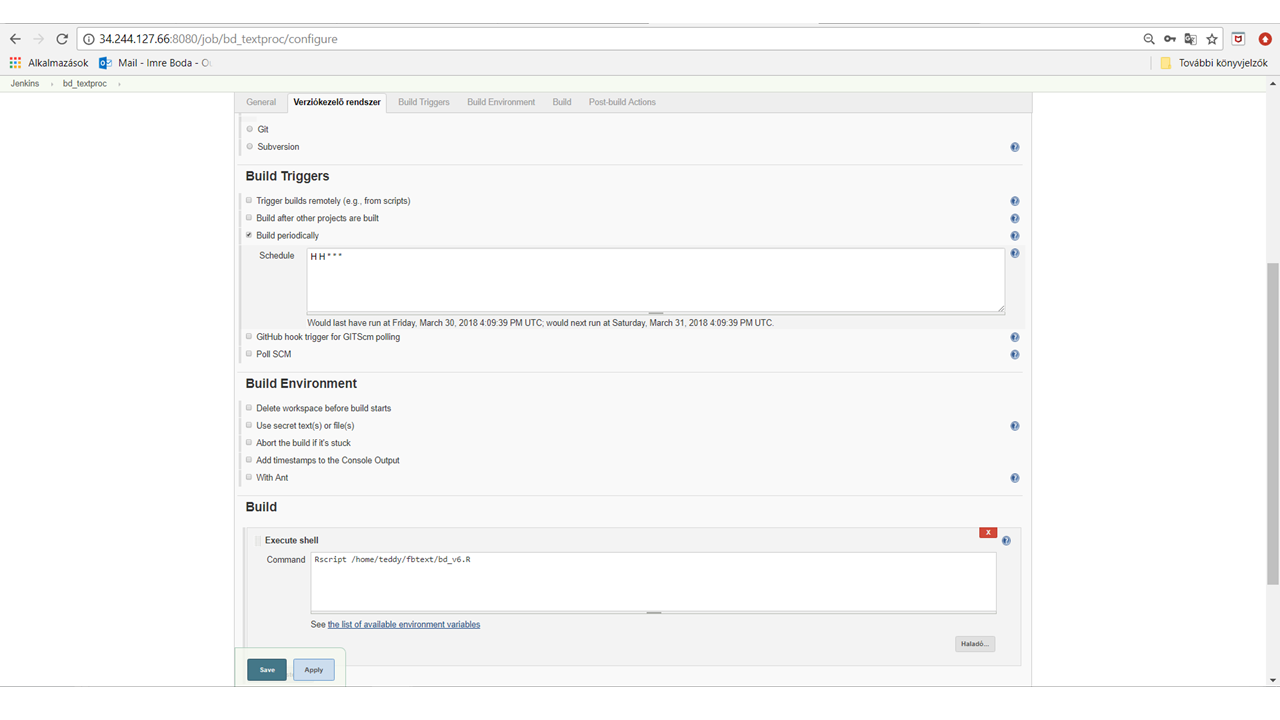
\includegraphics{/img/JenkinsSchedule.png}
\caption{Jenkins scheduler setting}
\end{figure}

\section{The shiny dashboard app}\label{the-shiny-dashboard-app}

The standard shiny Dashboard layout is used, which consists of a header,
a sidebar and a main body part.

The sidebar contains nothing else but a selectbox to choose the vendor
to be analyzed.

The body section consists of three parts:

\begin{itemize}
\tightlist
\item
  The upper part displays the key themes of the selected vendor by
  quarters. The most often used 5 ``real'' words and bi-grams are
  regarded as key topics, as described above.
\item
  The middle layer allows a quarter and a second vendor selection via
  two other selectboxes. The idea is to allow some comparison to reveal
  how similar or different two telco vendors' key themes are; to see if
  there are any significant differences between their slogans that might
  reveal different market strategy. So under the selectboxes the two
  vendors' key themes in the selected quarter are plotted (in
  wordcloud), and also a graph that displays the frequencies of the
  themes (words and bi-grams) used by both vendors. This graph reveals
  how many common themes these have in their posts (the more words
  presented on the plot), and also how much emphasis the vendors give to
  these themes (the closer the points are to the diagonal line, the more
  similar emphasis is given to a theme represented by the word/bi-gram),
\item
  The bottom part shows the sentiment score of the comments given to the
  vendors' posts by time.
\end{itemize}

The dashboard is written in a single app file, containing both the ui
and the server functions.

\paragraph{The input selectors}\label{the-input-selectors}

There are three selectbox inputs.

The first one allows to chose the ``main'' vendor. This is looked at in
all three dashboard sections.

Its selectbox is placed in the sidebar as shown below:

\begin{Shaded}
\begin{Highlighting}[]
\NormalTok{sidebar <-}\StringTok{ }\KeywordTok{dashboardSidebar}\NormalTok{(}
  
  \KeywordTok{selectInput}\NormalTok{(}\DataTypeTok{inputId =} \StringTok{"vendorselect"}\NormalTok{,}
              \DataTypeTok{label =} \StringTok{"Select Vendor"}\NormalTok{,}
              \DataTypeTok{choices =} \NormalTok{Vendor_list)}
  \NormalTok{)}
\end{Highlighting}
\end{Shaded}

Vendor\_list is read at the server start (in case of change in vendors,
it has to be restarted).

The second selector allows a ``comparison'' vendor to select, this is
the one whose market themes are compared to the ``main'' vendor's in the
middle section, and the comments' sentiments also in the bottom section.

Giving value to this is slightly more work than doing for the ``main''
vendor.

First, because here we need to make sure not to select the ``main''
vendor; the latter must be excluded from the list of selectable vendors.

Second, because simply excluding the ``main'' vendor from the selectable
list via ``choices = Vendor\_list {[}Vendor\_list !=
input\$vendorselect{]}'' results in an error message displayed at the
middle section's middle plot for about half a second. After that it
disappears, so not a big deal indeed, but still not nice. In order to
get rid of this disturbing error, a reactive variable is introduced,
which is first initialized with the second item on the vendors' list.
When the user selects a second vendor, this reactive variable is getting
new value. All plotting functions presenting anything about second
vendor will use this reactive variable, and not directly the output if
the input selector for the second vendor. This way these plotting
functions will always get non-NULL value.

\begin{Shaded}
\begin{Highlighting}[]
  \NormalTok{vendor2 <-}\StringTok{ }\KeywordTok{reactiveVal}\NormalTok{(Vendor_list [}\DecValTok{2}\NormalTok{]) }
  
  \NormalTok{output$select_vendor2 <-}\StringTok{ }\KeywordTok{renderUI}\NormalTok{(\{}
    \KeywordTok{selectInput}\NormalTok{(}\DataTypeTok{inputId =} \StringTok{"vendor2"}\NormalTok{,}
                \DataTypeTok{label =} \StringTok{"Select Another Vendor to compare"}\NormalTok{,}
                \DataTypeTok{choices =} \NormalTok{Vendor_list [Vendor_list !=}\StringTok{ }\NormalTok{input$vendorselect])}
  \NormalTok{\})}
  
  \KeywordTok{observeEvent}\NormalTok{(input$vendor2, \{}
    \KeywordTok{vendor2}\NormalTok{(input$vendor2)             }\CommentTok{# rv$value <- newValue}
  \NormalTok{\})}
\end{Highlighting}
\end{Shaded}

The third input selector allows picking the quarter for the theme
comparison in the middle section. It is a simple selectInput, the same
as in the sidebar, except that here the list to be selected from is the
list of quarters of the analysis period.

\paragraph{The output functions:
plots}\label{the-output-functions-plots}

\subparagraph{Top section}\label{top-section}

It is a simple ``jitter plot'' with the relative frequency of the word /
bi-gram on the y, and quarter on the x axis. The input is the top5 (top5
per word plus top5 per bi-gram, per quarter per vendor) results of the
post and comment reader and processor script.

\begin{Shaded}
\begin{Highlighting}[]
\NormalTok{output$plot1 <-}\StringTok{ }\KeywordTok{renderPlot}\NormalTok{(\{prop_top5 %>%}\StringTok{ }\KeywordTok{filter} \NormalTok{(Vendor ==}\StringTok{ }\NormalTok{input$vendorselect)%>%}
\StringTok{      }\KeywordTok{ggplot} \NormalTok{(}\KeywordTok{aes}\NormalTok{(created_Q, prop, }\DataTypeTok{color=}\NormalTok{created_Q, }\DataTypeTok{label =} \NormalTok{word)) +}\StringTok{ }\KeywordTok{geom_jitter} \NormalTok{(}\DataTypeTok{size =}\DecValTok{0}\NormalTok{) +}\StringTok{ }
\StringTok{      }\KeywordTok{geom_text_repel} \NormalTok{(}\DataTypeTok{size=}\DecValTok{5}\NormalTok{, }\DataTypeTok{segment.color =} \StringTok{"white"}\NormalTok{) +}\StringTok{ }\KeywordTok{theme_bw} \NormalTok{(}\DataTypeTok{base_size =} \DecValTok{24}\NormalTok{) +}\StringTok{ }
\StringTok{      }\KeywordTok{theme}\NormalTok{(}\DataTypeTok{legend.position=}\StringTok{"none"}\NormalTok{, }\DataTypeTok{panel.grid.major=}\KeywordTok{element_blank}\NormalTok{(),}
            \DataTypeTok{panel.grid.minor=}\KeywordTok{element_blank}\NormalTok{(), }\DataTypeTok{axis.text.y=}\KeywordTok{element_blank}\NormalTok{(), }\DataTypeTok{axis.line =} \KeywordTok{element_blank}\NormalTok{()) +}
\StringTok{      }\KeywordTok{labs}\NormalTok{(}\DataTypeTok{title =} \KeywordTok{sprintf} \NormalTok{(}\StringTok{"Most frequent themes in %s Facebook posts"}\NormalTok{, }\KeywordTok{toupper}\NormalTok{(input$vendorselect))) +}
\StringTok{           }\KeywordTok{xlab}\NormalTok{(}\StringTok{"Quarters"}\NormalTok{) +}\StringTok{ }\KeywordTok{ylab}  \NormalTok{(}\StringTok{"Frequency"}\NormalTok{)}
    \NormalTok{\})}
\end{Highlighting}
\end{Shaded}

\subparagraph{Middle section}\label{middle-section}

The two wordclouds at the two ends work pretty much the same way, except
that the one for the ``comparison'' vendor uses the reactive variable,
while the other one can take the result of its inputSelect directly.
They both work on the same data as the plot in the top section.

\begin{Shaded}
\begin{Highlighting}[]
  \NormalTok{output$cloud1 <-}\StringTok{ }\KeywordTok{renderPlot}\NormalTok{(\{}
    \NormalTok{prop_top5 %>%}\StringTok{ }\KeywordTok{filter} \NormalTok{(Vendor ==}\StringTok{ }\NormalTok{input$vendorselect) %>%}\StringTok{ }\KeywordTok{filter} \NormalTok{(created_Q ==}\StringTok{ }\NormalTok{input$quarterselect) %>%}
\StringTok{      }\KeywordTok{with}\NormalTok{(}\KeywordTok{wordcloud}\NormalTok{(word, n, }\DataTypeTok{max.words =} \DecValTok{100}\NormalTok{, }\DataTypeTok{min.freq =} \FloatTok{0.2}\NormalTok{, }\DataTypeTok{scale =} \KeywordTok{c}\NormalTok{(}\DecValTok{3}\NormalTok{,}\FloatTok{0.5}\NormalTok{), }\DataTypeTok{colors =} \KeywordTok{c}\NormalTok{(}\StringTok{"#0091ff"}\NormalTok{, }\StringTok{"#f0650e"}\NormalTok{)))  }
  \NormalTok{\})}
  \NormalTok{output$cloud2 <-}\StringTok{ }\KeywordTok{renderPlot}\NormalTok{(\{}
    \NormalTok{prop_top5 %>%}\StringTok{ }\KeywordTok{filter} \NormalTok{(Vendor ==}\StringTok{ }\KeywordTok{vendor2}\NormalTok{()) %>%}\StringTok{ }\KeywordTok{filter} \NormalTok{(created_Q ==}\StringTok{ }\NormalTok{input$quarterselect) %>%}\StringTok{ }
\StringTok{      }\KeywordTok{with}\NormalTok{(}\KeywordTok{wordcloud}\NormalTok{(word, n, }\DataTypeTok{max.words =} \DecValTok{100}\NormalTok{, }\DataTypeTok{min.freq =} \FloatTok{0.2}\NormalTok{, }\DataTypeTok{scale =} \KeywordTok{c}\NormalTok{(}\DecValTok{3}\NormalTok{,}\FloatTok{0.5}\NormalTok{),}\DataTypeTok{colors =} \KeywordTok{c}\NormalTok{(}\StringTok{"#0091ff"}\NormalTok{, }\StringTok{"#f0650e"}\NormalTok{)))  }
  \NormalTok{\})}
\end{Highlighting}
\end{Shaded}

The middle plot looks at the frequency table of all uni-grams and
bi-grams and plots it on a ``jitter plot''. For every word coming to the
plot the relative frequency in the ``comparison'' vendor's frequency
table is presented on the x axis, while on the y axis the same for the
``main'' vendor.

The scale is logarithmic, consequently, words and bi-grams that are
present in one but not in the other's posts are not even shown. This
means that the less points are on the displays, the less common themes
the vendors have. And as said above, the closer is a point to the
diagonal line, it has more similar frequency in the vendors' posts. In
an oversimple interpretation: getting the same focus.

\begin{Shaded}
\begin{Highlighting}[]
  \NormalTok{output$CompPlot <-}\StringTok{ }\KeywordTok{renderPlot} \NormalTok{(\{}
    \NormalTok{proportion %>%}
\StringTok{      }\KeywordTok{filter} \NormalTok{(created_Q ==}\StringTok{ }\NormalTok{input$quarterselect) %>%}
\StringTok{      }\KeywordTok{filter} \NormalTok{(Vendor %in%}\StringTok{ }\KeywordTok{c}\NormalTok{(input$vendorselect, }\KeywordTok{vendor2}\NormalTok{())) %>%}
\StringTok{      }\KeywordTok{select} \NormalTok{(-n) %>%}\StringTok{     }\CommentTok{#drop n, in order  to allow spread and collapse (gather)}
\StringTok{      }\KeywordTok{spread} \NormalTok{(Vendor, prop) %>%}\StringTok{    }\CommentTok{#spred prop per vendor}
\StringTok{      }\KeywordTok{gather} \NormalTok{(Vendor, prop, -created_Q, -word, -}\KeywordTok{c}\NormalTok{(input$vendorselect, }\KeywordTok{vendor2}\NormalTok{())) %>%}
\StringTok{      }\KeywordTok{ggplot} \NormalTok{( }\KeywordTok{aes}\NormalTok{(}\KeywordTok{get}\NormalTok{(}\KeywordTok{vendor2}\NormalTok{())/}\DecValTok{100}\NormalTok{, }\KeywordTok{get}\NormalTok{(input$vendorselect)/}\DecValTok{100}\NormalTok{, }
                   \DataTypeTok{color =} \KeywordTok{abs} \NormalTok{(}\KeywordTok{get}\NormalTok{(input$vendorselect)-}\KeywordTok{get}\NormalTok{(}\KeywordTok{vendor2}\NormalTok{())))) +}\StringTok{ }
\StringTok{      }\KeywordTok{geom_abline} \NormalTok{(}\DataTypeTok{color =} \StringTok{"gray40"}\NormalTok{, }\DataTypeTok{lty =}\DecValTok{2}\NormalTok{) +}\StringTok{ }
\StringTok{      }\KeywordTok{geom_jitter} \NormalTok{(}\DataTypeTok{alpha =} \FloatTok{0.3}\NormalTok{, }\DataTypeTok{size =} \FloatTok{2.5}\NormalTok{, }\DataTypeTok{width =} \FloatTok{0.3}\NormalTok{, }\DataTypeTok{height =} \FloatTok{0.3}\NormalTok{) +}
\StringTok{      }\KeywordTok{geom_text}\NormalTok{(}\KeywordTok{aes}\NormalTok{(}\DataTypeTok{label =} \NormalTok{word), }\DataTypeTok{check_overlap =} \OtherTok{TRUE}\NormalTok{, }\DataTypeTok{vjust =} \FloatTok{1.5}\NormalTok{) +}
\StringTok{      }\KeywordTok{scale_x_log10}\NormalTok{(}\DataTypeTok{labels =} \KeywordTok{percent_format}\NormalTok{(), }\DataTypeTok{limits =} \KeywordTok{c}\NormalTok{(}\FloatTok{0.001}\NormalTok{,}\FloatTok{0.1}\NormalTok{)) +}
\StringTok{      }\KeywordTok{scale_y_log10}\NormalTok{(}\DataTypeTok{labels =} \KeywordTok{percent_format}\NormalTok{(), }\DataTypeTok{limits =} \KeywordTok{c}\NormalTok{(}\FloatTok{0.001}\NormalTok{,}\FloatTok{0.1}\NormalTok{)) +}
\StringTok{      }\KeywordTok{scale_color_gradient}\NormalTok{(}\DataTypeTok{limits =} \KeywordTok{c}\NormalTok{(}\DecValTok{0}\NormalTok{, }\DecValTok{2}\NormalTok{), }\DataTypeTok{low =} \StringTok{"#0091ff"}\NormalTok{, }\DataTypeTok{high =} \StringTok{"#f0650e"}\NormalTok{) +}
\StringTok{      }\CommentTok{#facet_wrap (~ Vendor, ncol = 5) +}
\StringTok{      }\KeywordTok{theme_bw}\NormalTok{() +}\StringTok{ }\KeywordTok{theme}\NormalTok{(}\DataTypeTok{legend.position=}\StringTok{"none"}\NormalTok{) +}
\StringTok{      }\KeywordTok{labs}\NormalTok{(}\DataTypeTok{y =} \NormalTok{input$vendorselect, }\DataTypeTok{x =} \KeywordTok{vendor2}\NormalTok{())}
      
  \NormalTok{\})}
\end{Highlighting}
\end{Shaded}

At the beginning I planned to represent such similarity and
dissimilarity with commonality and comparison clouds from the same
``wordcloud'' package. However, it seemed not to be trivial how to cope
with cases when a message was in high focus at both vendors, but with
different weights. (e.g.~this was the case with Ericsson and ZTE: both
had 5G as their \#1 topic by far, but as in Ericsson's posts it appeared
with even higher frequency than in ZTE's, it was shown as a difference
between the two. Whereas the reality is that it was by far the most
exposed topic at both vendors, hence, it is a strong similarity in their
strategic focus, not dissimilarity).

I am sure that there is some nice way to overcome this, but for the sake
of time I decided to leave the cloud comparison for ``inside'' vendors'
topics and use this (visually less attractive) solution: cloud where
font sizes represent frequency among the given vendor's topics (not
across vendors).

\subparagraph{The bottom section}\label{the-bottom-section}

Finally, there come two highcharts to present the comments sentiment
scores for the two selected vendors: the upper one displays the ``main''
vendor's by time, the lower one the ``comparison'' vendor's. I picked
the ``stock'' type highchart for such display, because this creates
amazing timeline charts.

The two outputs are pretty much alike, the only notable difference is
that the second one uses here again the reactive variable, while the
main vendors' chart takes value from the relevant input selector
directly.

\begin{Shaded}
\begin{Highlighting}[]
\NormalTok{output$hc <-}\StringTok{ }\KeywordTok{renderHighchart}\NormalTok{(\{}
    \NormalTok{hc <-}\StringTok{ }\NormalTok{comment_sent %>%}\StringTok{ }
\StringTok{      }\KeywordTok{filter} \NormalTok{(Vendor ==}\StringTok{ }\NormalTok{input$vendorselect) %>%}\StringTok{ }
\StringTok{      }\KeywordTok{hchart}\NormalTok{(}\StringTok{"line"}\NormalTok{, }\KeywordTok{hcaes}\NormalTok{(}\DataTypeTok{x=}\KeywordTok{as.Date}\NormalTok{(}\StringTok{`}\DataTypeTok{as.Date(Comment_created_time)}\StringTok{`}\NormalTok{), }\DataTypeTok{y =} \NormalTok{sentiment)) %>%}\StringTok{        }
\StringTok{      }\KeywordTok{hc_xAxis}\NormalTok{(}\DataTypeTok{type =} \StringTok{"datetime"}\NormalTok{) %>%}
\StringTok{      }\KeywordTok{hc_title} \NormalTok{(}\DataTypeTok{text =} \KeywordTok{sprintf}\NormalTok{(}\StringTok{"Comments' sentiments of %s"}\NormalTok{, }\KeywordTok{toupper}\NormalTok{(input$vendorselect)))}
    \NormalTok{hc <-}\StringTok{ }\KeywordTok{hc_tooltip}\NormalTok{(hc, }\DataTypeTok{pointFormat =} \StringTok{"Daily Sentiment Score: \{point.y\}"}\NormalTok{)}
      
    \NormalTok{hc$x$type <-}\StringTok{ "stock"}                              \CommentTok{#"stock"}
    
    \NormalTok{hc}
    
  \NormalTok{\})}
  
  \NormalTok{output$hc2 <-}\StringTok{ }\KeywordTok{renderHighchart}\NormalTok{(\{}
    \NormalTok{hc2 <-}\StringTok{ }\NormalTok{comment_sent %>%}\StringTok{ }
\StringTok{      }\KeywordTok{filter} \NormalTok{(Vendor ==}\StringTok{ }\KeywordTok{vendor2}\NormalTok{()) %>%}\StringTok{ }
\StringTok{      }\KeywordTok{hchart}\NormalTok{(}\StringTok{"line"}\NormalTok{, }\KeywordTok{hcaes}\NormalTok{(}\DataTypeTok{x=}\KeywordTok{as.Date}\NormalTok{(}\StringTok{`}\DataTypeTok{as.Date(Comment_created_time)}\StringTok{`}\NormalTok{), }\DataTypeTok{y =} \NormalTok{sentiment)) %>%}\StringTok{        }
\StringTok{      }\KeywordTok{hc_xAxis}\NormalTok{(}\DataTypeTok{type =} \StringTok{"datetime"}\NormalTok{) %>%}
\StringTok{      }\KeywordTok{hc_title} \NormalTok{(}\DataTypeTok{text =} \KeywordTok{sprintf}\NormalTok{(}\StringTok{"Comments' sentiments of %s"}\NormalTok{, }\KeywordTok{toupper}\NormalTok{(}\KeywordTok{vendor2}\NormalTok{())))}
    \NormalTok{hc2 <-}\StringTok{ }\KeywordTok{hc_tooltip}\NormalTok{(hc2, }\DataTypeTok{pointFormat =} \StringTok{"Daily Sentiment Score: \{point.y\}"}\NormalTok{)}
    
    \NormalTok{hc2$x$type <-}\StringTok{ "stock"}                              \CommentTok{#"stock"}
    
    \NormalTok{hc2}
    
  \NormalTok{\})}
\end{Highlighting}
\end{Shaded}

\section{Conclusion}\label{conclusion}

Well, this was just a toy, but still it reveals some interesting things:

\begin{itemize}
\tightlist
\item
  First, telco vendors messages are more diverged than I expected. It
  looks that some are more willing to explore ``non traditional'' telco
  areas than others.
\item
  I found a lot of similarities between Ericsson and ZTE key themes in
  all quarters.
\item
  Even those who are not familiar with the telco business can conclude
  that the two major events of the industry are CES and MWC.
\item
  There is quite a big dissimilarity between the traditional telco
  vendor' messages and the others. Though telco and IT converge, it
  looks that telco vendors are more ``traditional'' than the benchmarked
  other players.
\item
  I had hard time concluding anything from the comment sentiment score
  graphs. Maybe as next step I will correlate the scores and messages of
  the same dates to see what caused extra peaks and drops.
\end{itemize}

\section{Annex}\label{annex}

Github repo: \url{https://github.com/imreboda/telco_text}


\end{document}
